\item \points{3di} {\bf Run Fine-Tuning with LoRA}

Run fine-tuning for each parameter-efficient fine-tuning method, using $p=4,16$ for LoRA (so, 5 variants in total); run the commands:

{\small \texttt{python3 main.py --task run\_ft --model med --mode first,last,middle,lora4,lora16 \textbackslash \\
\phantom{asdf}--dataset xsum,babi --k 0,1,8,128}}

Plot \textbf{k-shot performance} as \textbf{k is varied} for GPT-2-medium, one plot for each dataset; run the commands:

{\small \texttt{python3 main.py --task plot\_ft --model med --mode first,last,middle,lora4,lora16 \textbackslash \\
\phantom{asdf}--dataset xsum --k 0,1,8,128}}

Plot for the above is as follows:
\begin{center}
    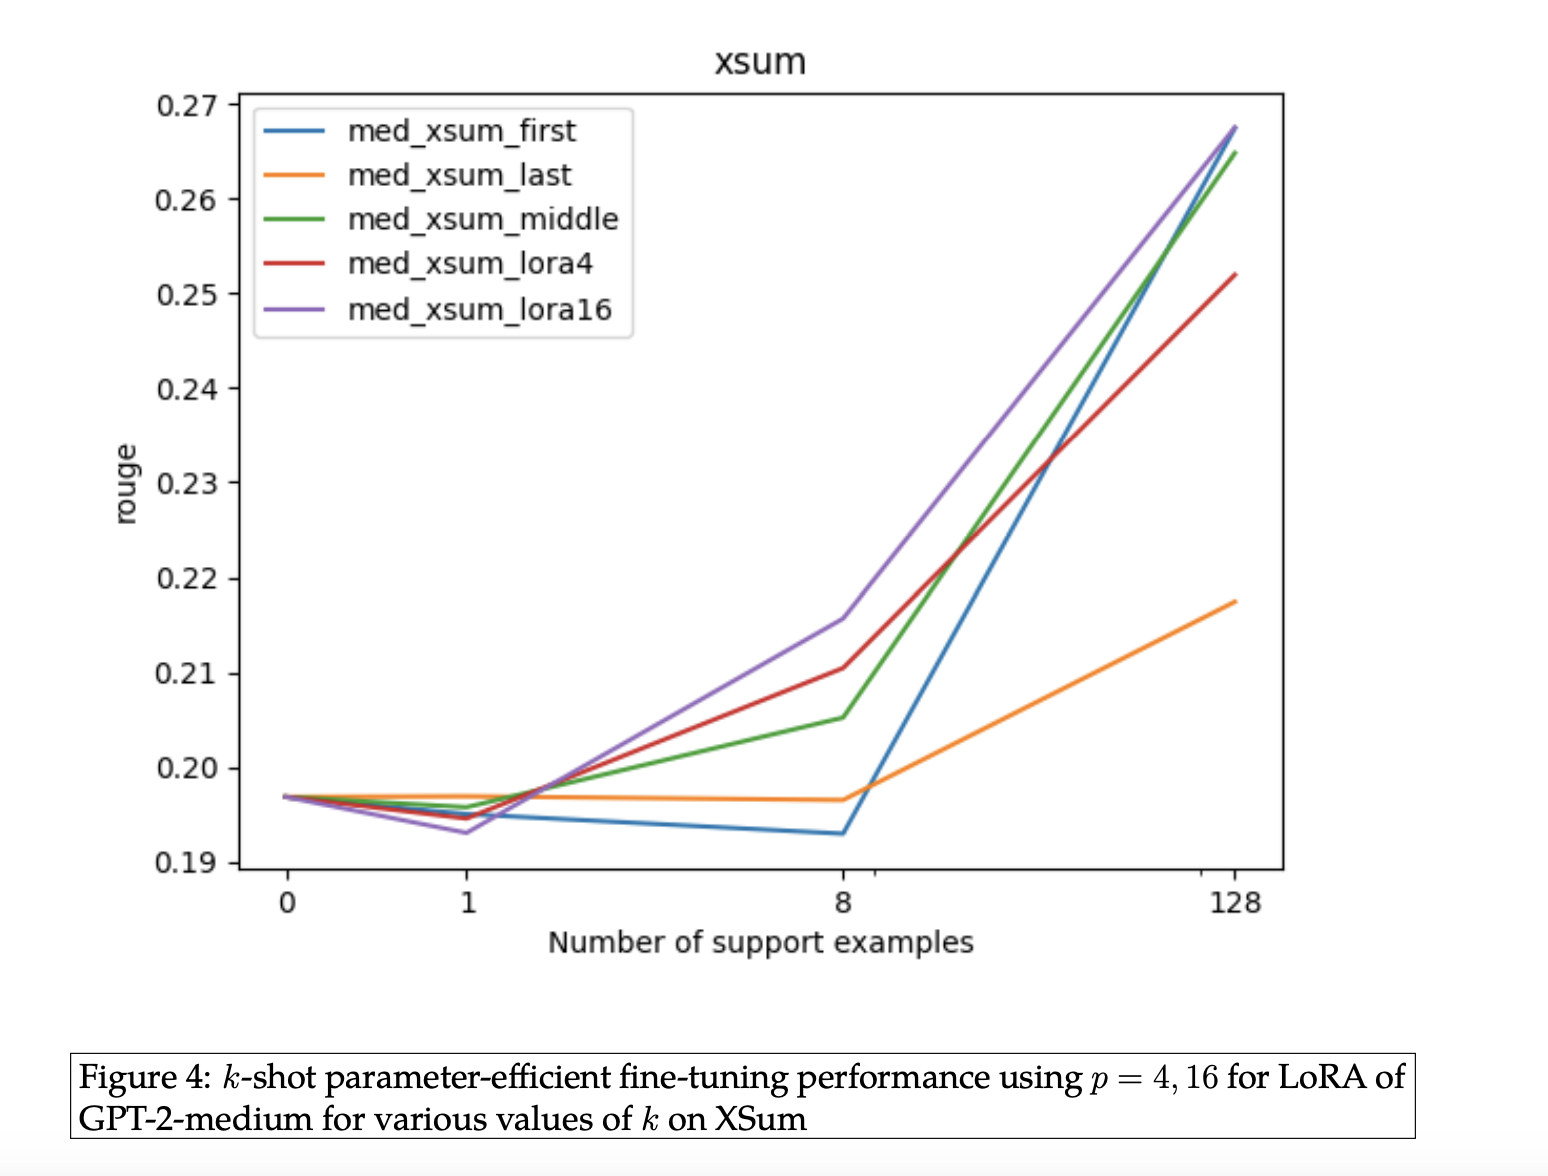
\includegraphics[width=0.75\linewidth]{./figures/parameter-3ci}
\end{center}

{\small \texttt{python3 main.py --task plot\_ft --model med --mode first,last,middle,lora4,lora16 \textbackslash \\
\phantom{asdf}--dataset babi --k 0,1,8,128}}

Plot for the above is as follows:
\begin{center}
    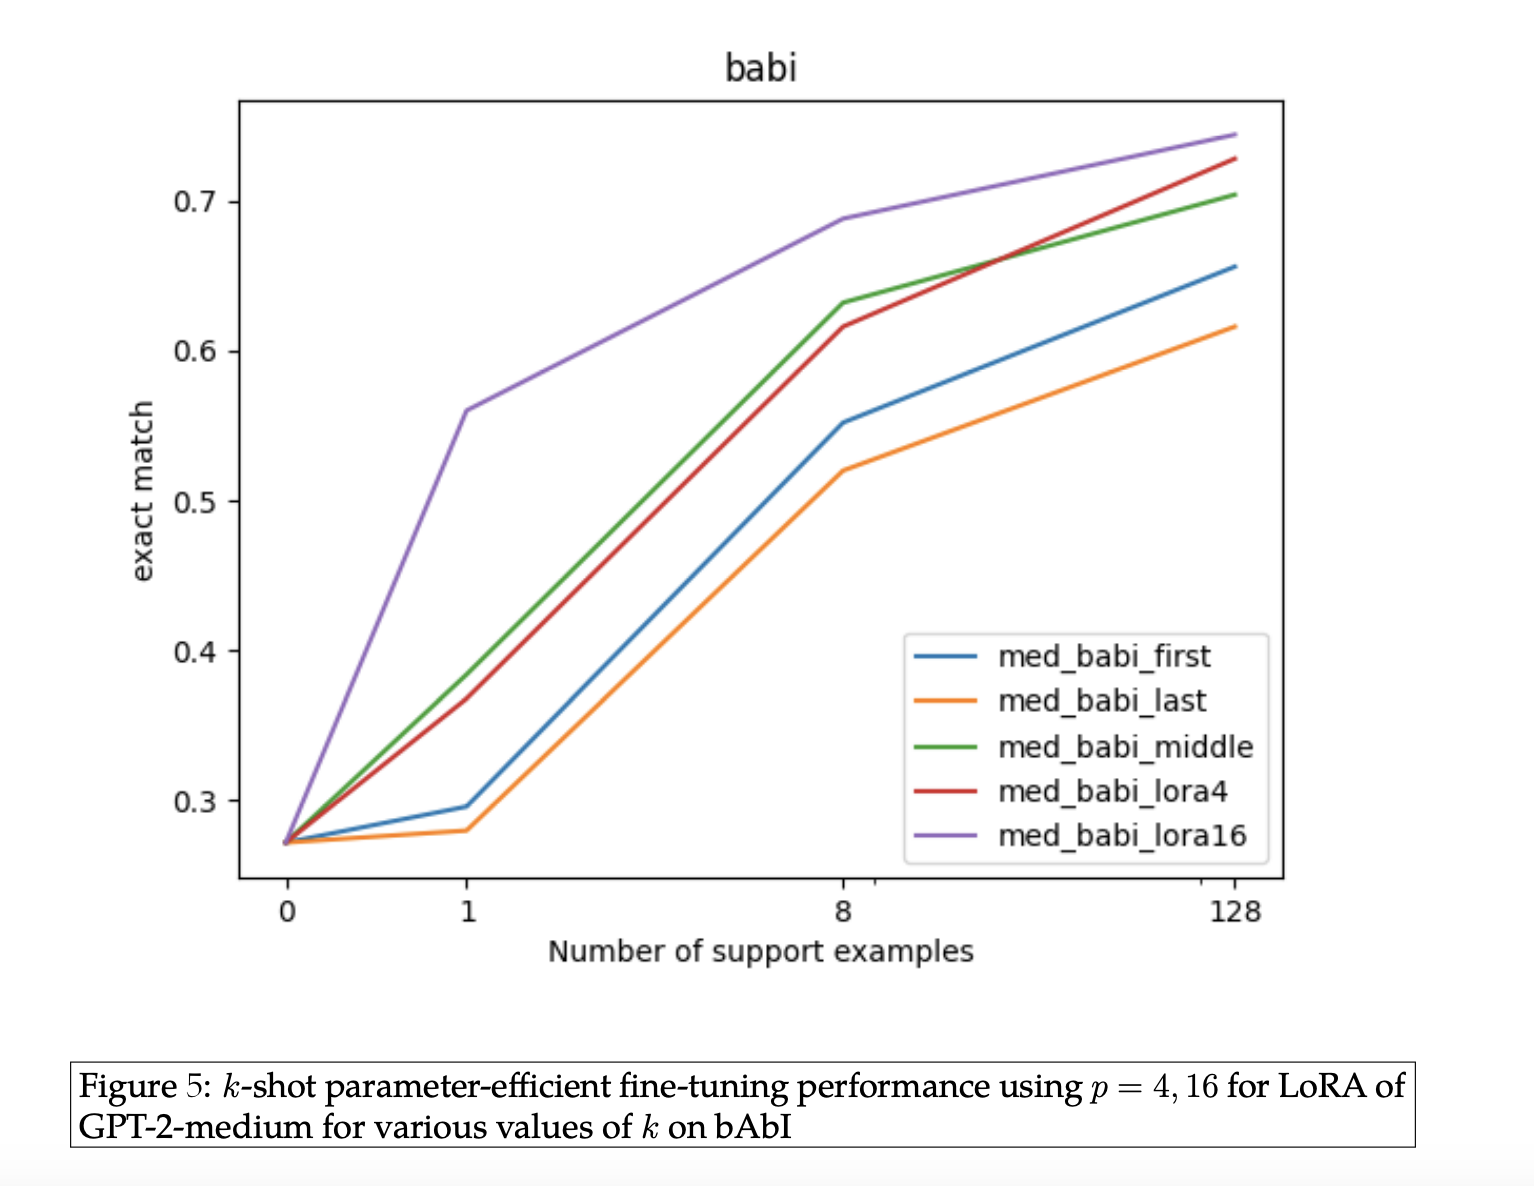
\includegraphics[width=0.75\linewidth]{./figures/parameter-3cii}
\end{center}
